\section{Study Diary}

This chapter holds our journal of lessons learned during the course. Detailed analysis of each Sprints' contents shall follow.

\subsection{Sprint 1}

\paragraph{} For this first sprint the product owner proposed a very minimalist approach as we familiarized ourselves with the several new tools at our disposal. The official requirement was to fulfill two user stories per sprint, and conveniently enough, the first two tasks were as simple as; one: reading input from the user (their name) and then two: printing out a personalized backstory for them.

\subsubsection{Everything went well (almost everything)}

\paragraph{} Right from the get go we had a very good understanding of how to achieve our goals. As such, it was easy to start working on the project and rapidly deliver outstanding results for the first sprint. In fact we completed our intentionally very light sprint 1 workload before it even officially began.

\paragraph{} As to not fall into despair from lack of work, we selected additional tasks to complete. In the end, we have four additional user stories more or less in a completed state, in addition to the first two proposed solutions that were refactored several times until they met everyone's ever higher standards for good code.

\subsubsection{We had difficulties}

\paragraph{Communication} Working in a team can be difficult, especially when it comes to communicating between team members. None of us were very familiar with Agilefant, so we did most of the communication on WhatsApp and in person.

\paragraph{Missed deadline} One failure was that we missed the delivery deadline. All our tasks were complete weeks ago, but we never submitted them to Repolainen because we constantly kept adding new things. In the future, we will create calendar entries for each deadline with automatic email notifications set up to give us a reminder two days in advance.

\subsubsection{What were the main learnings}

\paragraph{} We should use Agilefant more often, in order to make sure that we’re all on the same page. It also helps in defining clear objectives for individuals and for the team as a whole.

\subsubsection{For the next sprint, we decided to change...}

\paragraph{our work habits and one tool} We decided to try and take more advantage of the tools at our disposal. Since our team works mostly in quick and very productive iterations, it might be interesting for us to synchronize our efforts in real-life sprints.

\paragraph{} As we have had difficulties taming Microsoft Office, a proposed move to TeX was initiated. It will improve our work process greatly. No more crashes due to faulty edit conflict resolution, nor unnecessary struggling with the laggy online version of Word that performs especially poorly on MacBooks.

\subsection{Sprint 2}

\paragraph{} The goal of this sprint was to implement the core features of the game. Indeed, in order for our product to actually \emph{feel} like a game, we needed the notions of an objective and obstacles.

\subsubsection{All is well in the world}

\paragraph{} It's been smooth sailing on this sprint. With our experience working as a team with Agilefant and Processing, a lot of features we'd planned came together nicely.

\subsubsection{Difficulties?}

\paragraph{} The difficulties are really starting to show on the road that lies ahead. Some questions were brought up during this sprint that will only be answered during Sprint 3. Hopefully, the answers will not be too painful for us.

\paragraph{} One such question is the issue of performance. While performance is very dependent on the computer the game runs on, we noticed some frames dropped on the current version of the game. A situation that could get worse as we add more and more logic and objects on each game scene. Thus we will have to pay special attention to the related parts of the program to make sure the game still runs smoothly in the future.

\paragraph{} Some questions arose also about the exact satisfaction of the customer requirements. Will we fill the requirements exactly how they are presented, or change them slightly to create a better game?

\subsubsection{What we learned}

\paragraph{} Compared to Sprint 1, the learnings were much lighter this time around. Our skills in both Processing and Agilefant continued improving during the sprint. Additionally, we learned that we need to better take into account the future directions of the game.

\subsubsection{Moving on}

\paragraph{} While some features are best left to be implemented later, it is sometimes useful to prepare the road for future work. Some big architecture changes on this sprint should really ease the implementation of some of Sprint 3's user stories.

\paragraph{} However, more architecture changes will probably be needed later on.


\subsection{Sprint 3}

\paragraph{} This sprint focused on further refining the game, implementing almost all of the remaining user stories. Extra thought was put into our git workflow and the definition of done.

\paragraph{Git workflow} We are using a centralized workflow. This means we only have one master branch, which developers clone and commit to it. Centralized workflow is simple for the developers as long as conflicts are avoided. Since this is a small project and everyone is usually working at different times and different features, these problems rarely occur. Additionally, new features are simple enough that there is no need to commit non-working code and thus branches are generally not needed. Releases are marked with tags for Repolainen returns. Of course, some problems are possible: If two people try pushing at once, conflict happens. Also; always pull first, and then push. Resolve conflicts, if any. (Edit conflicts will arise if working on the same feature.)

\paragraph{Definition of Done} Although definition of done is not static, we have produced a list of features which indicate a user story is "Done". First of all, the code is completed, as in, all of the features which were to be done are produced in code. The code is pushed into the version control system and tested generally with the already existing features. The code is documented if necessary for the rest of the team to utilize it. Naturally, this means the code builds without errors and works as depicted from the story. The whole team approves of the addition, and the task hours are up to date and the estimated time left is set to zero in Agilefant.


\subsubsection{General feelings}

\paragraph{} A lot of time was spent discussing the features and the workflow. This pushed the actual implementation of the features quite late, but with teamwork everything is possible, and we managed to get them done just like we wanted in this sprint.

\subsubsection{What we learned}

\paragraph{} We learned to use Agilefant even better than before, and to define our workflow and the "Done". Our skills in Processing improved further as we implemented new features to our game.

\paragraph{Meta-learning} The learnings on sprints have largely been retrospective based on the things that went well and the things that did not go so well. The learnings have been discussed in the group to find the biggest problems in each sprint and how to improve the work in the future. We have so far managed to greatly improve our Agilefant performance based on the feedback we have received in each sprint as well as having a better grasp on the project in general.

\subsubsection{For the next sprint...}

\paragraph{} For the next sprint, we should again pay attention to distributing the work involving the decisions in the game and development process and the actual development more evenly with each other, and not one part first, second part later -style. We are continually improving our Agilefant workflow.

\subsubsection{Burndown graphs comparison}

\paragraph{} After learning how to log our spent effort properly in sprint 3, our graphs became less jagged. Yes, Agilefant does not decrease remaining effort automatically. We have to do it by hand. And the moment we mark a task as done, all "effort left" on it is lost — reset to zero. Something to keep in mind for Sprint 4. \textit{Log effort first, mark as done second.} But I digress; the following images depict how we enhanced our reporting technique:

\begin{figure}[H]
\centering
\caption{At first, we were quite ''blocky''.} % 3ICE: Caption moved above figure (to help with pagination)
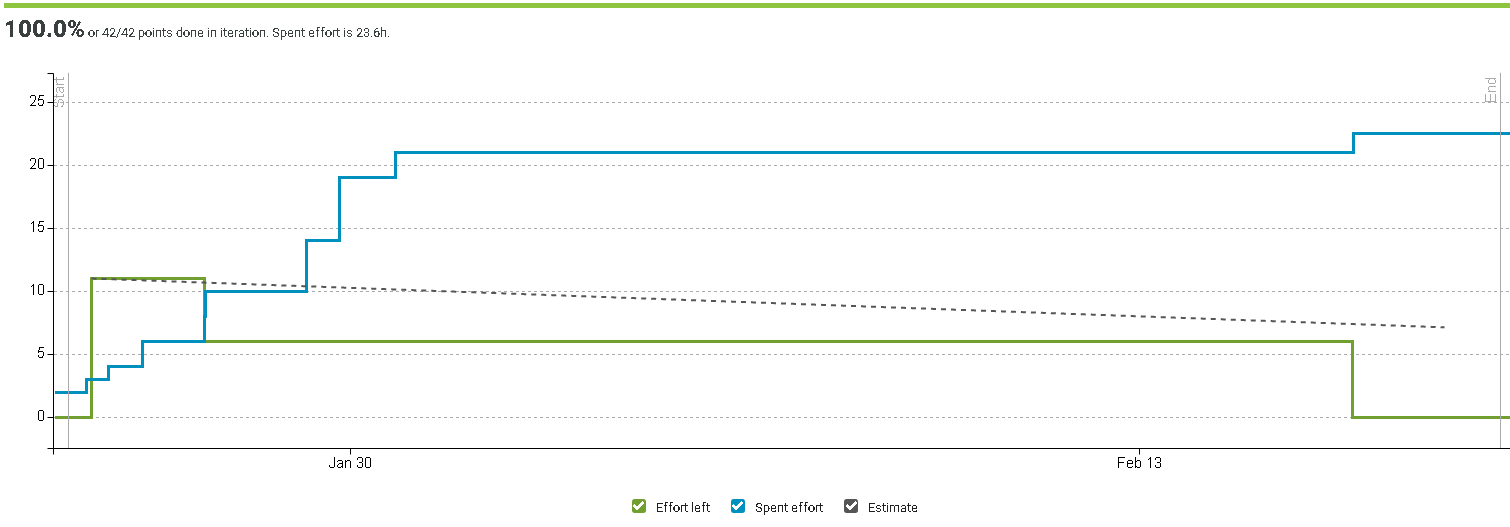
\includegraphics[width=\textwidth]{sprint1}
\end{figure}

And we were finished with everything before the sprint even officially began.

\begin{figure}[H]
\centering
\caption{Then we fine-grained the effort spent portion of the graph (blue).}
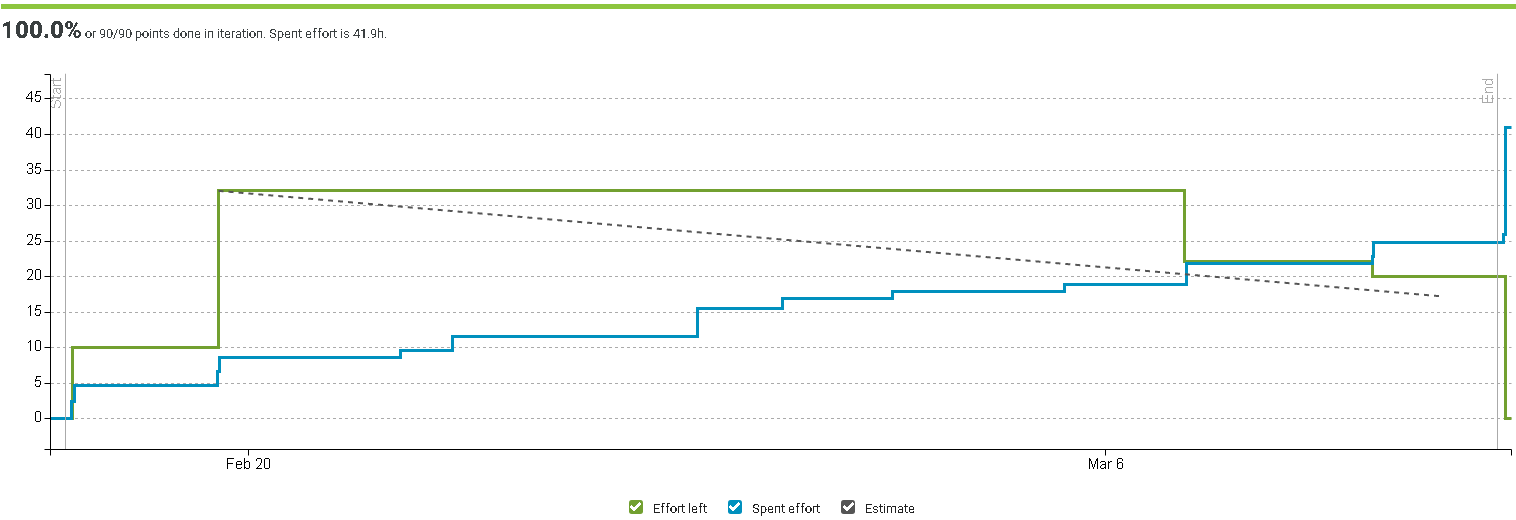
\includegraphics[width=\textwidth]{sprint2}
\end{figure}

\begin{figure}[H]
\centering
\caption{Finally, even the effort left portion is starting to look more detailed (green).}
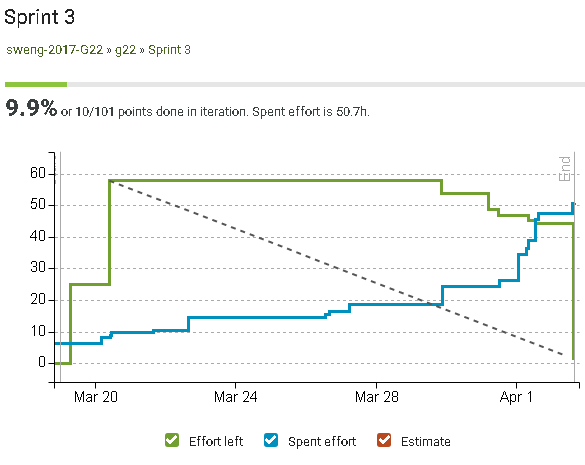
\includegraphics[width=\textwidth]{sprint3} % 3ICE: Update this picture before the deadline. Mark everything done to avoid showing only as 9.9% finished when in fact we're 100% done.
\end{figure}

\begin{figure}[H]
\centering
\caption{And here is an overview of the entire project. Significant improvement in Sprint 3 as we assign points to tasks more accurately.}
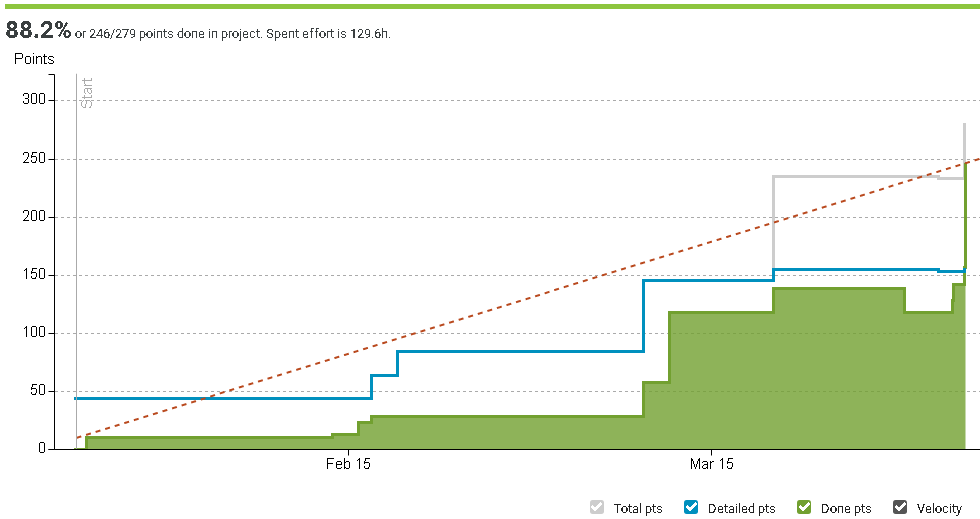
\includegraphics[width=\textwidth]{overview}
\end{figure}

\subsection{Sprint 4}

\paragraph{} This sprint focused on even further defining the game, implementing the last user stories and even some extra.

\subsubsection{General feelings}

\paragraph{} Sprint 4 went quite smoothly, as we were already experienced with both the project topic and the used tools; Processing, Git and Agilefant.

\subsubsection{What we learned}

\paragraph{} We learned to finally do appropriate logging in Agilefant. There were some difficulties with connectivity to the Agilefant server, but otherwise everything related that went smoothly. Code quality and refactoring was especially relevant to our work, since we were starting to have lots of game code made for the game we built the last features on, which meant we had to understand the code of other team members (and ourselves for a couple of months ago) as well.

\paragraph{Reviews} of the code were done at the end of the sprint, similarly to the last sprint. This was done commit-based through Git. Especial attention to them was paid this time as it was one of the sprint learning goals. We discussed the code on WhatsApp as well as utilized the GitLab comment feature. Everyone was expected to test their own code as usual, as well as a planned test before presenting the project.

\subsubsection{Burndown Chart}

\subsection{The whole project}

Overall, this has been a very educational project for all of the group members. Some of us were already experienced in game development before this course, so this in particular has not been the main thing we learned as a group. Most of us were also familiar with Git beforehand. Instead, we have learned a lot about agile development, especially the sprint system and the effort logging. Additionally, we learned how to look at the information we have generated through the system to see main contributors as well as how to interpret the burndown chart. This helped us better our estimations and the whole workflow. Still, some of the team was not as experienced in programming and thus learned a lot about it as well, as well as Processing as a language: some of us hadn't used Java before, and Processing was new to all of us. It was certainly an useful thing to learn as well, although it was also noticed that Processing is definitely not too suitable for larger projects.





 



